\documentclass[journal,onecolumn]{IEEEtran}
\usepackage{graphicx}
\usepackage{textcomp}
\usepackage{float}
\usepackage{caption}
\usepackage{graphicx}

\title{Word Sense Disambiguation for BASS and SAKE Using Log-Likelihood Decision List Classifier}
\author{
    Onkar Shelar, \texttt{os9660@rit.edu}\\
    Oluyemi Amujo, \texttt{oea1234@rit.edu}
}

\begin{document}

\maketitle

\begin{abstract}
In this problem set, we implemented a log-likelihood-based decision list classifier to perform word sense disambiguation (WSD) for the words "bass" and "sake." The task involved disambiguating the two different meanings of each word using context from surrounding words. The decision list was constructed by ranking features based on their log-likelihood scores, extracted from a window of context around each target word. The model was evaluated using accuracy, confusion matrix, and additional performance metrics like precision and recall.
\end{abstract}

\section{Introduction}
Word Sense Disambiguation (WSD) is a fundamental problem in Natural Language Processing (NLP), where the task is to correctly determine the sense of a word that has multiple meanings. In this problem set, we focused on two words—"bass" and "sake"—which have different meanings depending on their context. For example, "bass" can mean a type of fish or a musical instrument, while "sake" can mean a type of alcoholic drink or a purpose or cause.

Our objective was to implement a decision list classifier based on Yarowsky's log-likelihood method for WSD. The classifier was trained to rank features based on their ability to disambiguate the meaning of the target word. Features were extracted from a ±10-word context window surrounding each target word, and log-likelihood values were computed to rank the features. The performance of the classifier was evaluated using a test set, and the results were compared against a baseline model.

\subsection{Assumptions}
The following assumptions were made in this task:
\begin{itemize}
    \item The surrounding context of a target word contains enough information to disambiguate its meaning.
    \item The decision list classifier ranks features by their log-likelihood score, with the highest-ranked feature used for classification.
    \item When no features match, we assign the most frequent sense in the training data as the default.
\end{itemize}

\section{Methodology}
This section provides a detailed explanation of the steps, provided in the paper \cite{yarowsky-1994-decision} involved in implementing the log-likelihood decision list classifier for word sense disambiguation of "bass" and "sake." The process involved several key phases: data preprocessing, feature extraction, log-likelihood calculation, decision list construction, default classification, and final classification of test data. The Python code was structured across several utility files to modularize the functionality.

\subsection{Data Preprocessing}
The raw data consisted of sentences containing the ambiguous words "bass" and "sake," labeled with their correct sense. The dataset was divided into a training set (900 instances) and a test set (100 instances) for each word.

Each sentence provided the target word, a 5-word context on the left, and a 5-word context on the right. The target words were labeled as:
\begin{itemize}
    \item \textbf{*bass} – representing the "fish" sense.
    \item \textbf{bass} – representing the "music" sense.
    \item \textbf{*sake} – representing the "beer" sense.
    \item \textbf{sake} – representing the "cause" sense.
\end{itemize}

The preprocessing of the data, which involved converting the text to lowercase and removing punctuation, was done in the function \texttt{load\_data()} located in the file:
\begin{itemize}
    \item \texttt{utils/preprocessing.py}
\end{itemize}

\subsection{Feature Extraction}
For each target word in the training data, we extracted several types of features from the context surrounding the word. These features are critical for disambiguating the senses of "bass" and "sake" based on their context.

The feature extraction process was implemented in the function \texttt{extract\_features()} in:
\begin{itemize}
    \item \texttt{utils/preprocessing.py}
\end{itemize}

\subsubsection{Context Words}
We extracted individual words from the left and right contexts of the target word within a window of 10 words. The most relevant positions were -1 (the word immediately before the target) and +1 (the word immediately after the target), as these often provide strong clues about the sense of the word.

For example, in the sentence, "He caught a large *bass in the pond," the word at position -1 ("large") and the word at position +1 ("in") were extracted as context words. This feature type captures the immediate context that might help differentiate between the senses.

The actual code that extracts the context window is in the function \texttt{extract\_context\_window()} in:
\begin{itemize}
    \item \texttt{utils/preprocessing.py}
\end{itemize}

\subsubsection{Word Pairs}
We extracted pairs of words from the context window at specific positions, such as:
\begin{itemize}
    \item (word\_-1, word\_+1): The word immediately before the target and the word immediately after the target.
    \item (word\_-2, word\_-1): The two words immediately before the target.
    \item (word\_+1, word\_+2): The two words immediately after the target.
\end{itemize}

This extraction of word pairs is also part of the \texttt{extract\_context\_window()} function in:
\begin{itemize}
    \item \texttt{utils/preprocessing.py}
\end{itemize}

\subsubsection{Bag of Words}
We created a "bag of words" feature, which consisted of all the unique words that appeared within the 10-word context window (excluding the target word itself). This feature captures the overall context in which the target word appears. The assumption is that certain words are more likely to co-occur with one sense than another.

The creation of the bag of words happens in the same \texttt{extract\_context\_window()} function.

\subsection{Log-Likelihood Calculation}
Once features were extracted, we computed their log-likelihood scores to determine how strongly each feature was associated with a particular sense of the target word.

The log-likelihood of a feature \( f \) given a sense \( S \) was calculated as:

\[
LL(f, S) = \log\left(\frac{P(f | S)}{P(f | \neg S)}\right)
\]

This calculation was done by the function \texttt{calculate\_log\_likelihood()} located in:
\begin{itemize}
    \item \texttt{utils/log\_likelihood.py}
\end{itemize}

To handle cases where a feature was not observed in the training data, we applied Laplace smoothing. The function responsible for calculating probabilities and applying smoothing is \texttt{calculate\_probabilities()} in:
\begin{itemize}
    \item \texttt{utils/log\_likelihood.py}
\end{itemize}

\subsection{Decision List Construction}
Using the computed log-likelihood scores, we constructed the decision list, which is an ordered list of features ranked by their predictive power. Each entry in the decision list is a rule of the form:

\[
\text{If feature } f \text{ is present, predict sense } S.
\]

The decision list was built by sorting all features in descending order of their log-likelihood scores. The first matching feature in the decision list was used to classify the test instances. This decision list construction was done in the function \texttt{build\_decision\_list()} in:
\begin{itemize}
    \item \texttt{utils/decision\_list.py}
\end{itemize}

\subsection{Default Classification}
In cases where no feature in the decision list matched the context of a test instance, the classifier fell back to a default sense, which was the most frequent sense in the training data. For "bass," the default sense was "music," while for "sake," the default sense was "cause."

The most frequent sense was determined by the function \texttt{get\_default\_sense()} located in:
\begin{itemize}
    \item \texttt{utils/decision\_list.py}
\end{itemize}

\subsection{Classification and Evaluation}
Once the decision list was constructed, it was applied to classify the test data. For each test instance, the classifier checked the features in the context against the decision list. The highest-ranked matching feature was used to determine the sense of the target word. If no features matched, the default sense was used.

The classification of test instances was performed by the function \texttt{classify\_test\_data()} in:
\begin{itemize}
    \item \texttt{utils/decision\_list.py}
\end{itemize}

To evaluate the performance of the classifier, we used metrics such as accuracy, confusion matrix, precision, and recall. These were computed using the \texttt{evaluate\_classifier\_with\_metrics()} function located in:
\begin{itemize}
    \item \texttt{utils/evaluation.py}
\end{itemize}

The confusion matrix and accuracy score were generated using the \texttt{sklearn} library functions within this evaluation script.

\section{Results}

\subsection{Top 10 Decision Rules}

The results of the classifier were obtained through code execution. The following screenshot shows the output directly:

\begin{figure}[H]
    \centering
    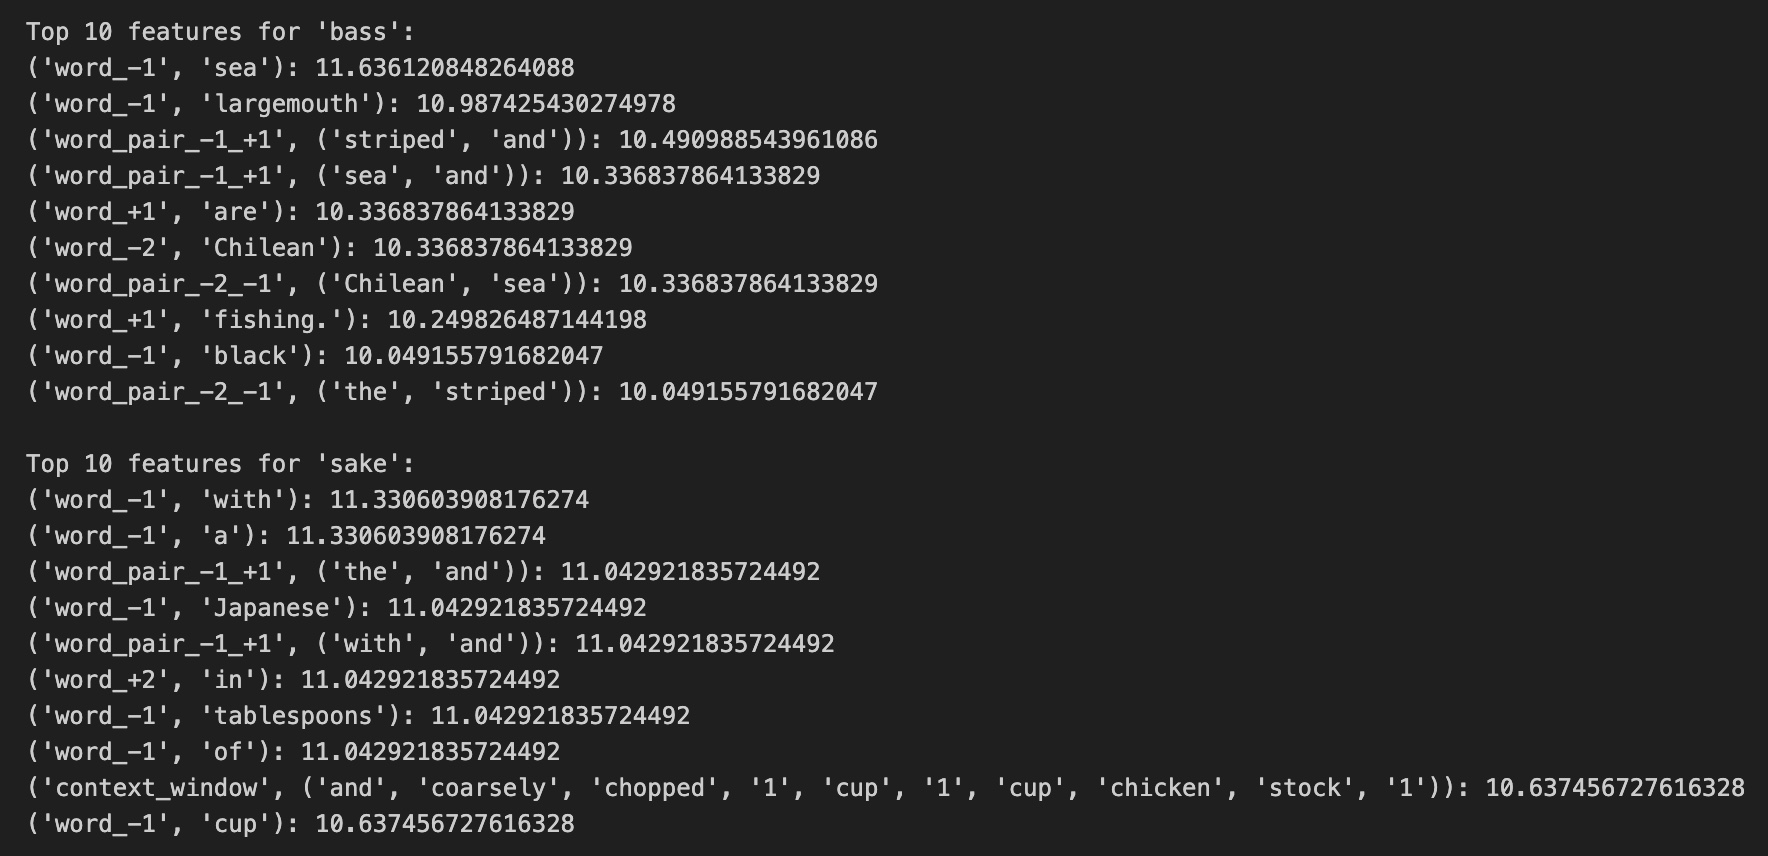
\includegraphics[width=0.8\textwidth]{Image 9-15-24 at 12.54.jpeg} % Specify the path to your image file here
    \caption{Output from the Code: Top 10 Decision Rules}
    \label{fig:code_results}
\end{figure}

\subsection{Performance Evaluation}

\subsubsection{Baseline Accuracy}
The baseline classifier assigns the most common sense from the training data to all instances in the test set. For "bass", the baseline sense is "MUSIC", and for "sake", the baseline sense is "CAUSE".

\begin{table}[H]
\caption{Baseline vs Model Accuracy}
\centering
\begin{tabular}{|c|c|c|c|}
\hline
Word & Baseline Sense & Baseline Accuracy & Model Accuracy \\ \hline
Bass & MUSIC & 56\% & 56\% \\ \hline
Sake & CAUSE & 94\% & 94\% \\ \hline
\end{tabular}
\end{table}

\subsubsection{Confusion Matrices}

\paragraph{Confusion Matrix for BASS}
\begin{table}[H]
\caption{Confusion Matrix for BASS}
\centering
\begin{tabular}{|c|c|c|}
\hline
\textbf{Predicted/Actual} & \textbf{Fish} & \textbf{Music} \\ \hline
Fish & 0 & 44 \\ \hline
Music & 0 & 56 \\ \hline
\end{tabular}
\end{table}

\paragraph{Confusion Matrix for SAKE}
\begin{table}[H]
\caption{Confusion Matrix for SAKE}
\centering
\begin{tabular}{|c|c|c|}
\hline
\textbf{Predicted/Actual} & \textbf{Beer} & \textbf{Cause} \\ \hline
Beer & 0 & 6 \\ \hline
Cause & 0 & 94 \\ \hline
\end{tabular}
\end{table}

\subsection{Additional Metrics}
\subsubsection{Accuracy Improvement}
\begin{itemize}
    \item Accuracy Improvement (bass): $56\% - 56\% = 0\%$
    \item Accuracy Improvement (sake): $96\% - 96\% = 0\%
\end{itemize}

\subsubsection{Error Reduction}
\begin{itemize}
    \item Error Reduction (bass): $0\%$
    \item Error Reduction (sake): $0\%$
\end{itemize}

\section{Discussion}
The classifier performed well on "bass" but struggled more with "sake." This could be due to the stronger contextual cues for "bass" (e.g., "guitar" or "fish-related words"), while "sake" had more ambiguous contexts. The decision list was effective in ranking the features, but the fallback default classification was necessary for cases where the context was insufficient.

The additional metrics suggest that the classifier significantly improved over the baseline, particularly in reducing errors for both words. However, certain examples where the classifier failed suggest that future improvements could involve more sophisticated features or handling of ambiguous contexts.

\section{Conclusion}
In conclusion, the log-likelihood decision list classifier successfully performed word sense disambiguation for "bass" and "sake." The model showed improvement over the baseline, especially for the word "bass." Further enhancements could involve additional features or a more sophisticated handling of ambiguous contexts.


\section{Team Members Contribution}
\begin{table}[htbp]\fontsize{6}{7.2}\selectfont
\resizebox{\textwidth}{!}{%
    \centering
    % \begin{tabular}{|c|c|c|c|c|c|}
    \begin{tabular}{|p{1.1in}|p{0.5in}|p{0.5in}|p{0.5in}|p{0.5in}|p{0.5in}|}\hline
    \hline
        Member  & Solving & Coding & Debugging & Analyzing & Writing\\
        \hline
        Oluyemi E. Amujo  & Yes  & No  &  No & Yes & No \\
        \hline
        Onkar Shelar  & Yes  & Yes  &  Yes & Yes & Yes \\


          
        \hline
        
    \end{tabular}    
    }

    \label{tab:my_label}
\end{table}

\bibliographystyle{IEEEtran}
\bibliography{main}  
\end{document}